\section{Evaluation}\label{sec:txid-evaluation}

\begin{outline}
  \item setup: both instantiations in Go over BLS12-381, gnark-crypto v0.21.0 (groups, pairing), gnark v0.16.3 (Groth16 circuits) (cite gnark-crypto)
  \item machine: MacBook Air, Apple M2, 16GB RAM
  \item method: 10 warm-up calls, 100 timed repetitions, report the median; IQR typically within 2\% of the median, never above 7\%
  \item headline $\ell = 8$, so $\Max = 256$ transactions per user per epoch
  \item point to \Cref{tab:txid-protocol,tab:txid-sizes,tab:txid-relations} (every algorithm, message, relation) and \Cref{fig:txid-ell-times,fig:txid-ell-sizes} (growth with $\ell$)
\end{outline}

\begin{table}[htbp] \centering \small
\caption[Tracing: time of every algorithm]{Time of each algorithm at $\ell = 8$, in milliseconds. A first grant is the first grant of a user to a given auditor, and
carries $\{W_\gamma\}$ in the algebraic instantiation. In the hash-based
instantiation every grant is the same.} \label{tab:txid-protocol}
  %
  \begin{tabular}{l l r r} \toprule
    %
    Algorithm & Party & Algebraic (ms) & Hash-based (ms) \\
    %
    \midrule
    %
    $\IDgen$ & & 2.50 & 267 \\
    %
    $\IDregister$ & user & 46.0 & 0.298 \\
    %
    $\IDregister$ & registration authority & 0.552 & 0.475 \\
    %
    $\IDgrant$, first & user & 4.22 & 17.3 \\
    %
    $\IDgrant$, first & auditor & 9.07 & 4.16 \\
    %
    $\IDgrant$, later & user & 0.689 & 17.3 \\
    %
    $\IDgrant$, later & auditor & 2.04 & 4.16 \\
    %
    $\IDsubmit$ & user & 11.3 & 28.3 \\
    %
    $\algo{Verify}$ & validator & 6.70 & 4.44 \\
    %
    $\IDidentify$, one epoch & auditor & 36.9 & 1.10 \\
    %
  \bottomrule \end{tabular}
%
\end{table}

\begin{table}[htbp] \centering \small
\caption[Tracing: message sizes]{Message sizes at $\ell = 8$, in bytes. A transaction includes a 32 byte
payload and its 8 byte length. Registration is three rounds and a grant two, in
each case starting with a 32 byte nonce from the registration authority or the
auditor.} \label{tab:txid-sizes}
  %
  \begin{tabular}{l r r} \toprule
    %
    Object & Algebraic (B) & Hash-based (B) \\
    %
    \midrule
    %
    Registration request (user) & 288 & 256 \\
    %
    Credential (registration authority) & 112 & 112 \\
    %
    $\PTK$ & 24\,624 & 48 \\
    %
    First grant message (user) & 25\,280 & 852 \\
    %
    Later grant message (user) & 608 & 852 \\
    %
    \midrule
    %
    Tag $\Tag_\gamma$ & 576 & 32 \\
    %
    Commitment $\com$ & 48 & 48 \\
    %
    Proof of $\rel_6'$, or $\rel_6$ & 544 & 512 \\
    %
    Proof of $\rel_7'$, or $\rel_7$ with its link & 3\,312 & 292 + 192 \\
    %
    Range proof & 640 & -- \\
    %
    Transaction & 5\,160 & 1\,116 \\
    %
  \bottomrule \end{tabular}
%
\end{table}

\begin{table}[htbp] \centering \small
\caption[Tracing: cost of each relation]{Time of each proof at $\ell = 8$, in milliseconds,
together with the Groth16 setups and circuit sizes of the hash-based
instantiation.} \label{tab:txid-relations}
  %
  \begin{tabular}{l l l r r} \toprule
    %
    Relation & Party & Frequency & Algebraic (ms) & Hash-based (ms) \\
    %
    \midrule
    %
    $\rel_4$ & prover & registration, grant & 0.228 & 0.151 \\
    %
    $\rel_4$ & verifier & registration, grant & 0.381 & 0.303 \\
    %
    $\rel_5$ & prover & grant & 0.451 & 16.8 \\
    %
    $\rel_5$ & verifier & grant & 0.597 & 2.24 \\
    %
    $\rel_5$ with $\{W_\gamma\}$ & prover & first grant & 4.00 & -- \\
    %
    $\rel_5$ with $\{W_\gamma\}$ & verifier & first grant & 7.64 & -- \\
    %
    $\rel_6'$, or $\rel_6$ & prover & transaction & 1.31 & 1.16 \\
    %
    $\rel_6'$, or $\rel_6$ & verifier & transaction & 1.79 & 1.69 \\
    %
    $\rel_7'$, or $\rel_7$ & prover & transaction & 3.96 & 26.5 \\
    %
    $\rel_7'$, or $\rel_7$ & verifier & transaction & 4.05 & 2.27 \\
    %
    Range proof & prover & transaction & 4.82 & -- \\
    %
    Range proof & verifier & transaction & 0.809 & -- \\
    %
    \midrule
    %
    $\rel_5$ setup & & deployment & -- & 95.3 \\
    %
    $\rel_7$ setup & & deployment & -- & 165 \\
    %
    $\rel_5$, $\rel_7$ constraints & & & -- & 668 and 1\,343 \\
    %
  \bottomrule \end{tabular}
%
\end{table}

\begin{figure}[htbp] \centering
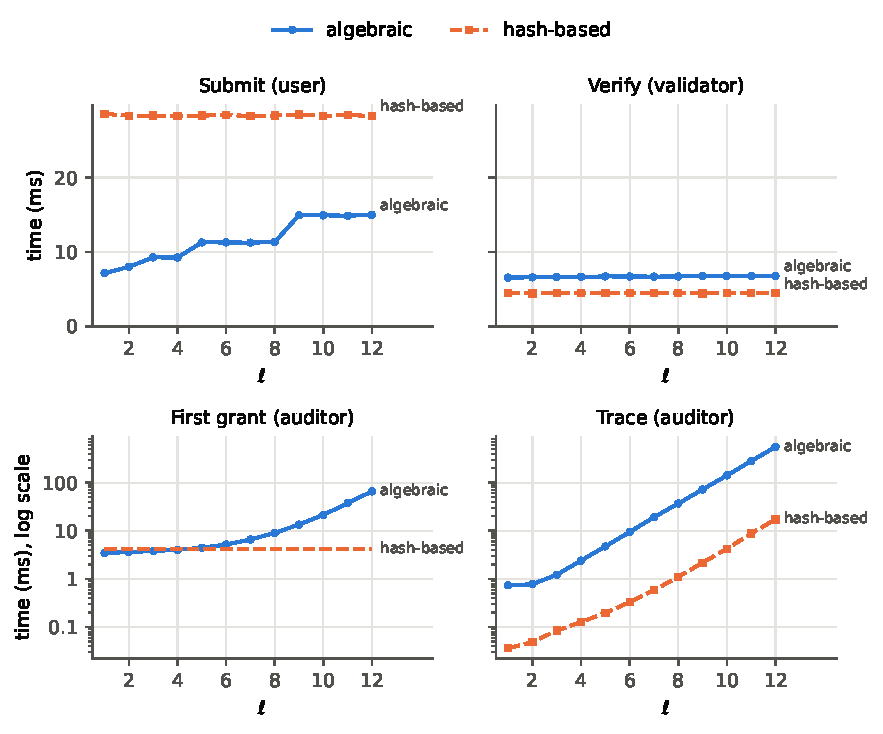
\includegraphics[width=\textwidth]{chapters/05-txid/txid-ell-times.pdf}
\caption[Tracing: time against $\ell$]{Time against $\ell$ for $\IDsubmit$, $\algo{Verify}$, the first grant as
verified by the auditor, and tracing one epoch. The first grant and tracing grow
with $\Max = 2^\ell$ and are on a log scale.} \label{fig:txid-ell-times}
\end{figure}

\begin{figure}[htbp] \centering
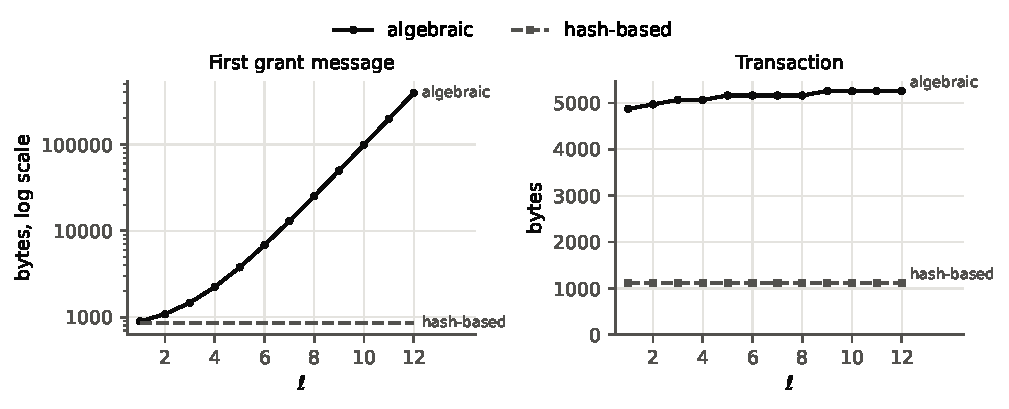
\includegraphics[width=0.75\textwidth]{chapters/05-txid/txid-ell-sizes.pdf}
\caption[Tracing: sizes against $\ell$]{Size against $\ell$ of the first grant message, on a log scale, and of
a transaction.} \label{fig:txid-ell-sizes} \end{figure}

\begin{outline}
  \item transaction: algebraic 11.3ms prove / 6.70ms verify; hash-based 28.3ms / 4.44ms, and a fifth of the size
  \item algebraic: the $\group{T}$ tag is the largest item on the ledger; torus compression would halve it
  \item verification and transaction size nearly flat in $\ell$; algebraic proving steps up just after each power of two (range proof pads to next power of two), hence $\ell = 8$ as headline
  \item first grant and tracing grow with $\Max = 2^\ell$, but tracing one user for one epoch never depends on ledger size or number of users: 36.9ms and 1.10ms at $\ell = 8$
\end{outline}

\begin{table}[htbp] \centering \small
\caption[Tracing against Idemix]{Per-transaction time in milliseconds and size in bytes, against Hyperledger Idemix, at $\ell = 8$. Idemix sizes are its own serialisation, with
uncompressed group elements.} \label{tab:txid-idemix}
  %
  \begin{tabular}{l r r r} \toprule
    %
    System & Prove (ms) & Verify (ms) & Size (B) \\
    %
    \midrule
    %
    Idemix, no oversight mechanism & 3.37 & 2.39 &
1\,099 \\
    %
    Idemix, with audit pseudonyms & 3.97 & 3.06 &
1\,535 \\
    %
    \midrule
    %
    This chapter, algebraic & 11.3 & 6.70 & 5\,160 \\
    %
    This chapter, hash-based & 28.3 & 4.44 & 1\,116 \\
    %
  \bottomrule \end{tabular}
%
\end{table}

\begin{outline}
  \item Idemix: Camenisch-Lysyanskaya line of credentials (cite CCS:CamVan02); run over the same library; \Cref{tab:txid-idemix} compares a transaction with an Idemix signature, with and without audit pseudonyms
  \item Idemix audits by testing one ledger entry at a time, 0.189ms per entry on one core, and only for signers who hand over their commitment randomness
  \item our tracing (eight cores) breaks even at about 200 entries per epoch (algebraic) and 6 (hash-based); at $10^6$ entries 37ms against 189s
\end{outline}
